\section{Hypothesis} %4.1
\label{section4.1}
\subsection{Hardware Hypothesis} %4.1.1
\label{subsection4.1.1}

In this Chapter, we use the algorithms described in the Chapter~\ref{Chapter3} to test the well-known Nordic system. One-line diagram of the Nordic test system is  shown in Figure~\ref{4_1_1_nordic}. 

\begin{figure}[htbp]
\centering
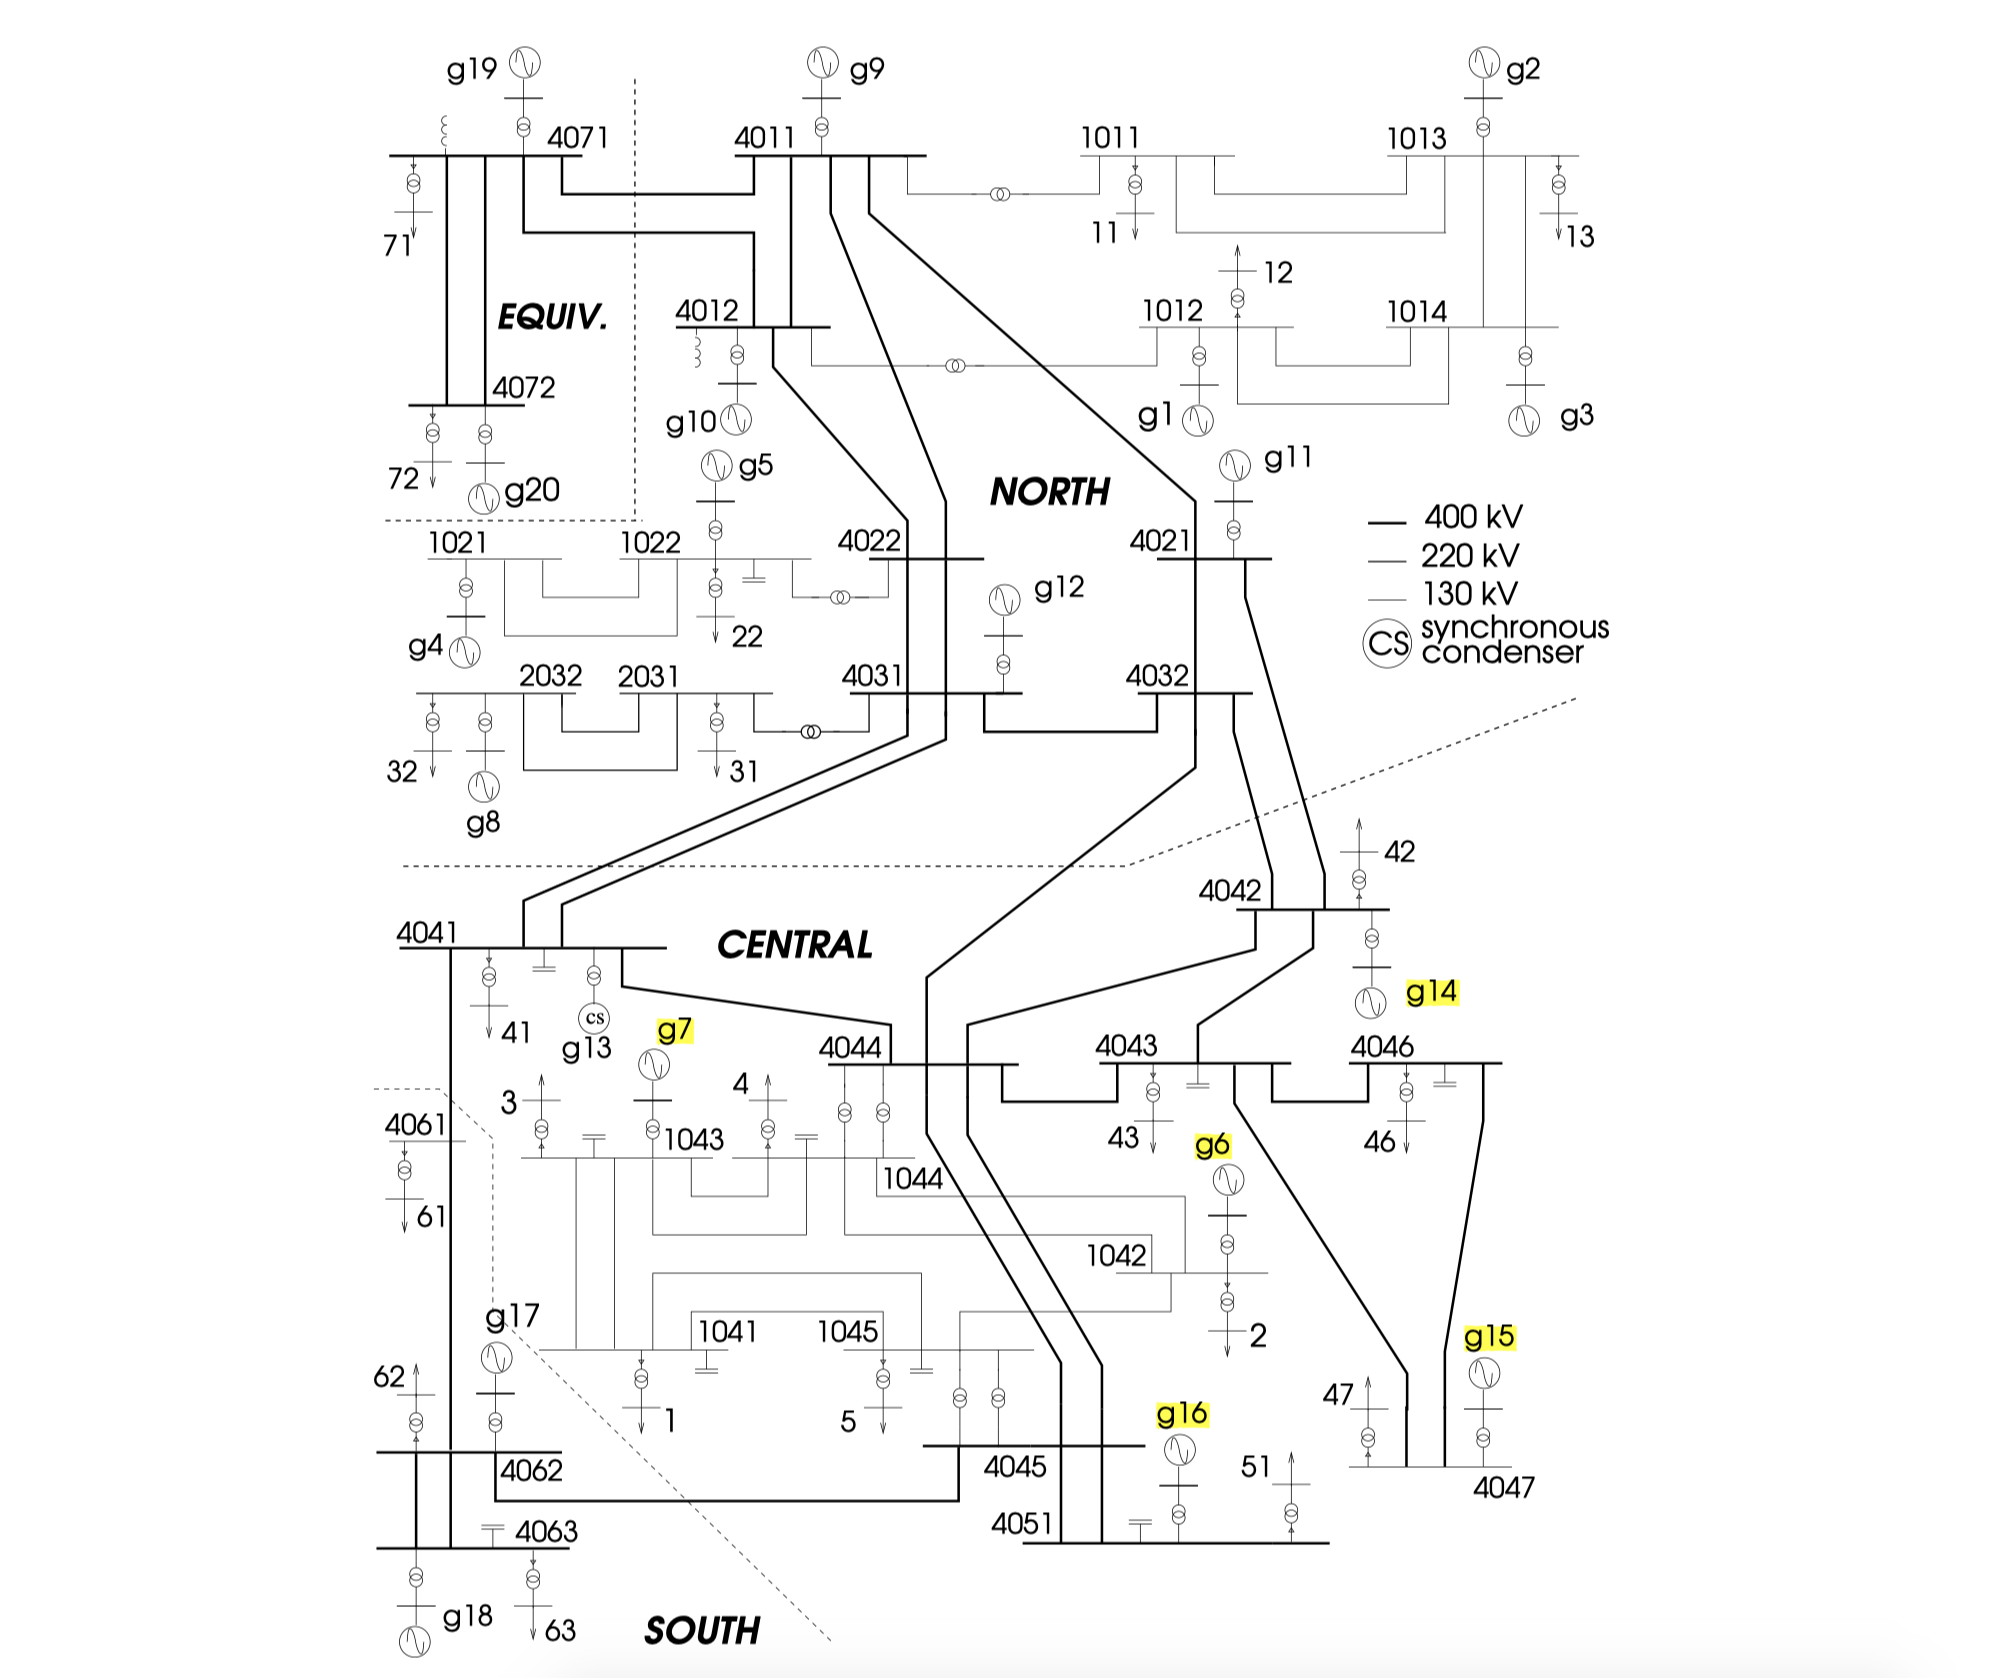
\includegraphics[width = .891\textwidth]{figure/4_1_1_nordic.png}
\caption{One-line diagram of the test system}
\label{4_1_1_nordic}
\end{figure}

Firstly, we assume g2 as our monitor. The monitor sends its frequency, also the frequency in the system, to the communication layer. Then, we choose five thermal generators  (g6, g7, g14, g15, g16) in the CENTRAL area. There are three reasons I choose these five generators that produce the power to the system when disturbances occur in the system. First of all, these are thermal generators not the generators in the NORTH area which are equipped with hydraulic turbines. We only have strict mathematical proof of thermal generators. Another reason is they have nice nominal power as shown the Table~\ref{nominalPower} below. The second reason is the difference of them is up to 900 MW which is good for researching the function of generators comprehensively. The last reason is I was collaborated with a PhD student. We researched Nordic test system in different algorithms. He used distributed method and I used centralised method. For convenience, we keep our generators the same. 


\begin{table}[htbp]
\centering
\begin{tabular}{ll}
Generator & Nominal Power (MW) \\
g1        & 760.0              \\
g2        & 570.0              \\
g3        & 665.0              \\
g4        & 570.0              \\
g5        & 237.5              \\
g6        & 360.0 (1/8)        \\
g7        & 180.0 (1/16)       \\
g8        & 807.5              \\
g9        & 950.0              \\
g10       & 760.0              \\
g11       & 285.0              \\
g12       & 332.5              \\
g13       & 0.0                \\
g14       & 630.0 (7/32)       \\
g15       & 1080.0 (3/8)       \\
g16       & 630.0 (7/32)       \\
g17       & 540.0              \\
g18       & 1080.0             \\
g19       & 475.0              \\
g20       & 4275.0             

\end{tabular}
\caption{Generators Nominal Power in Nordic.}
\label{nominalPower}
\end{table}

After choosing the generators, we need to choose a breaker. The breaker is a generator that can be disconnected to the system. Thus, a breaker is one of the most important impact factors to the grid system. However, at first, I am not sure how to choose a suitable breaker but then I try to disconnect all of them one by one without Secondary Frequency Control. Results are as Figure~\ref{4_1_1_without1}. 

\begin{figure}[htbp]
\centering
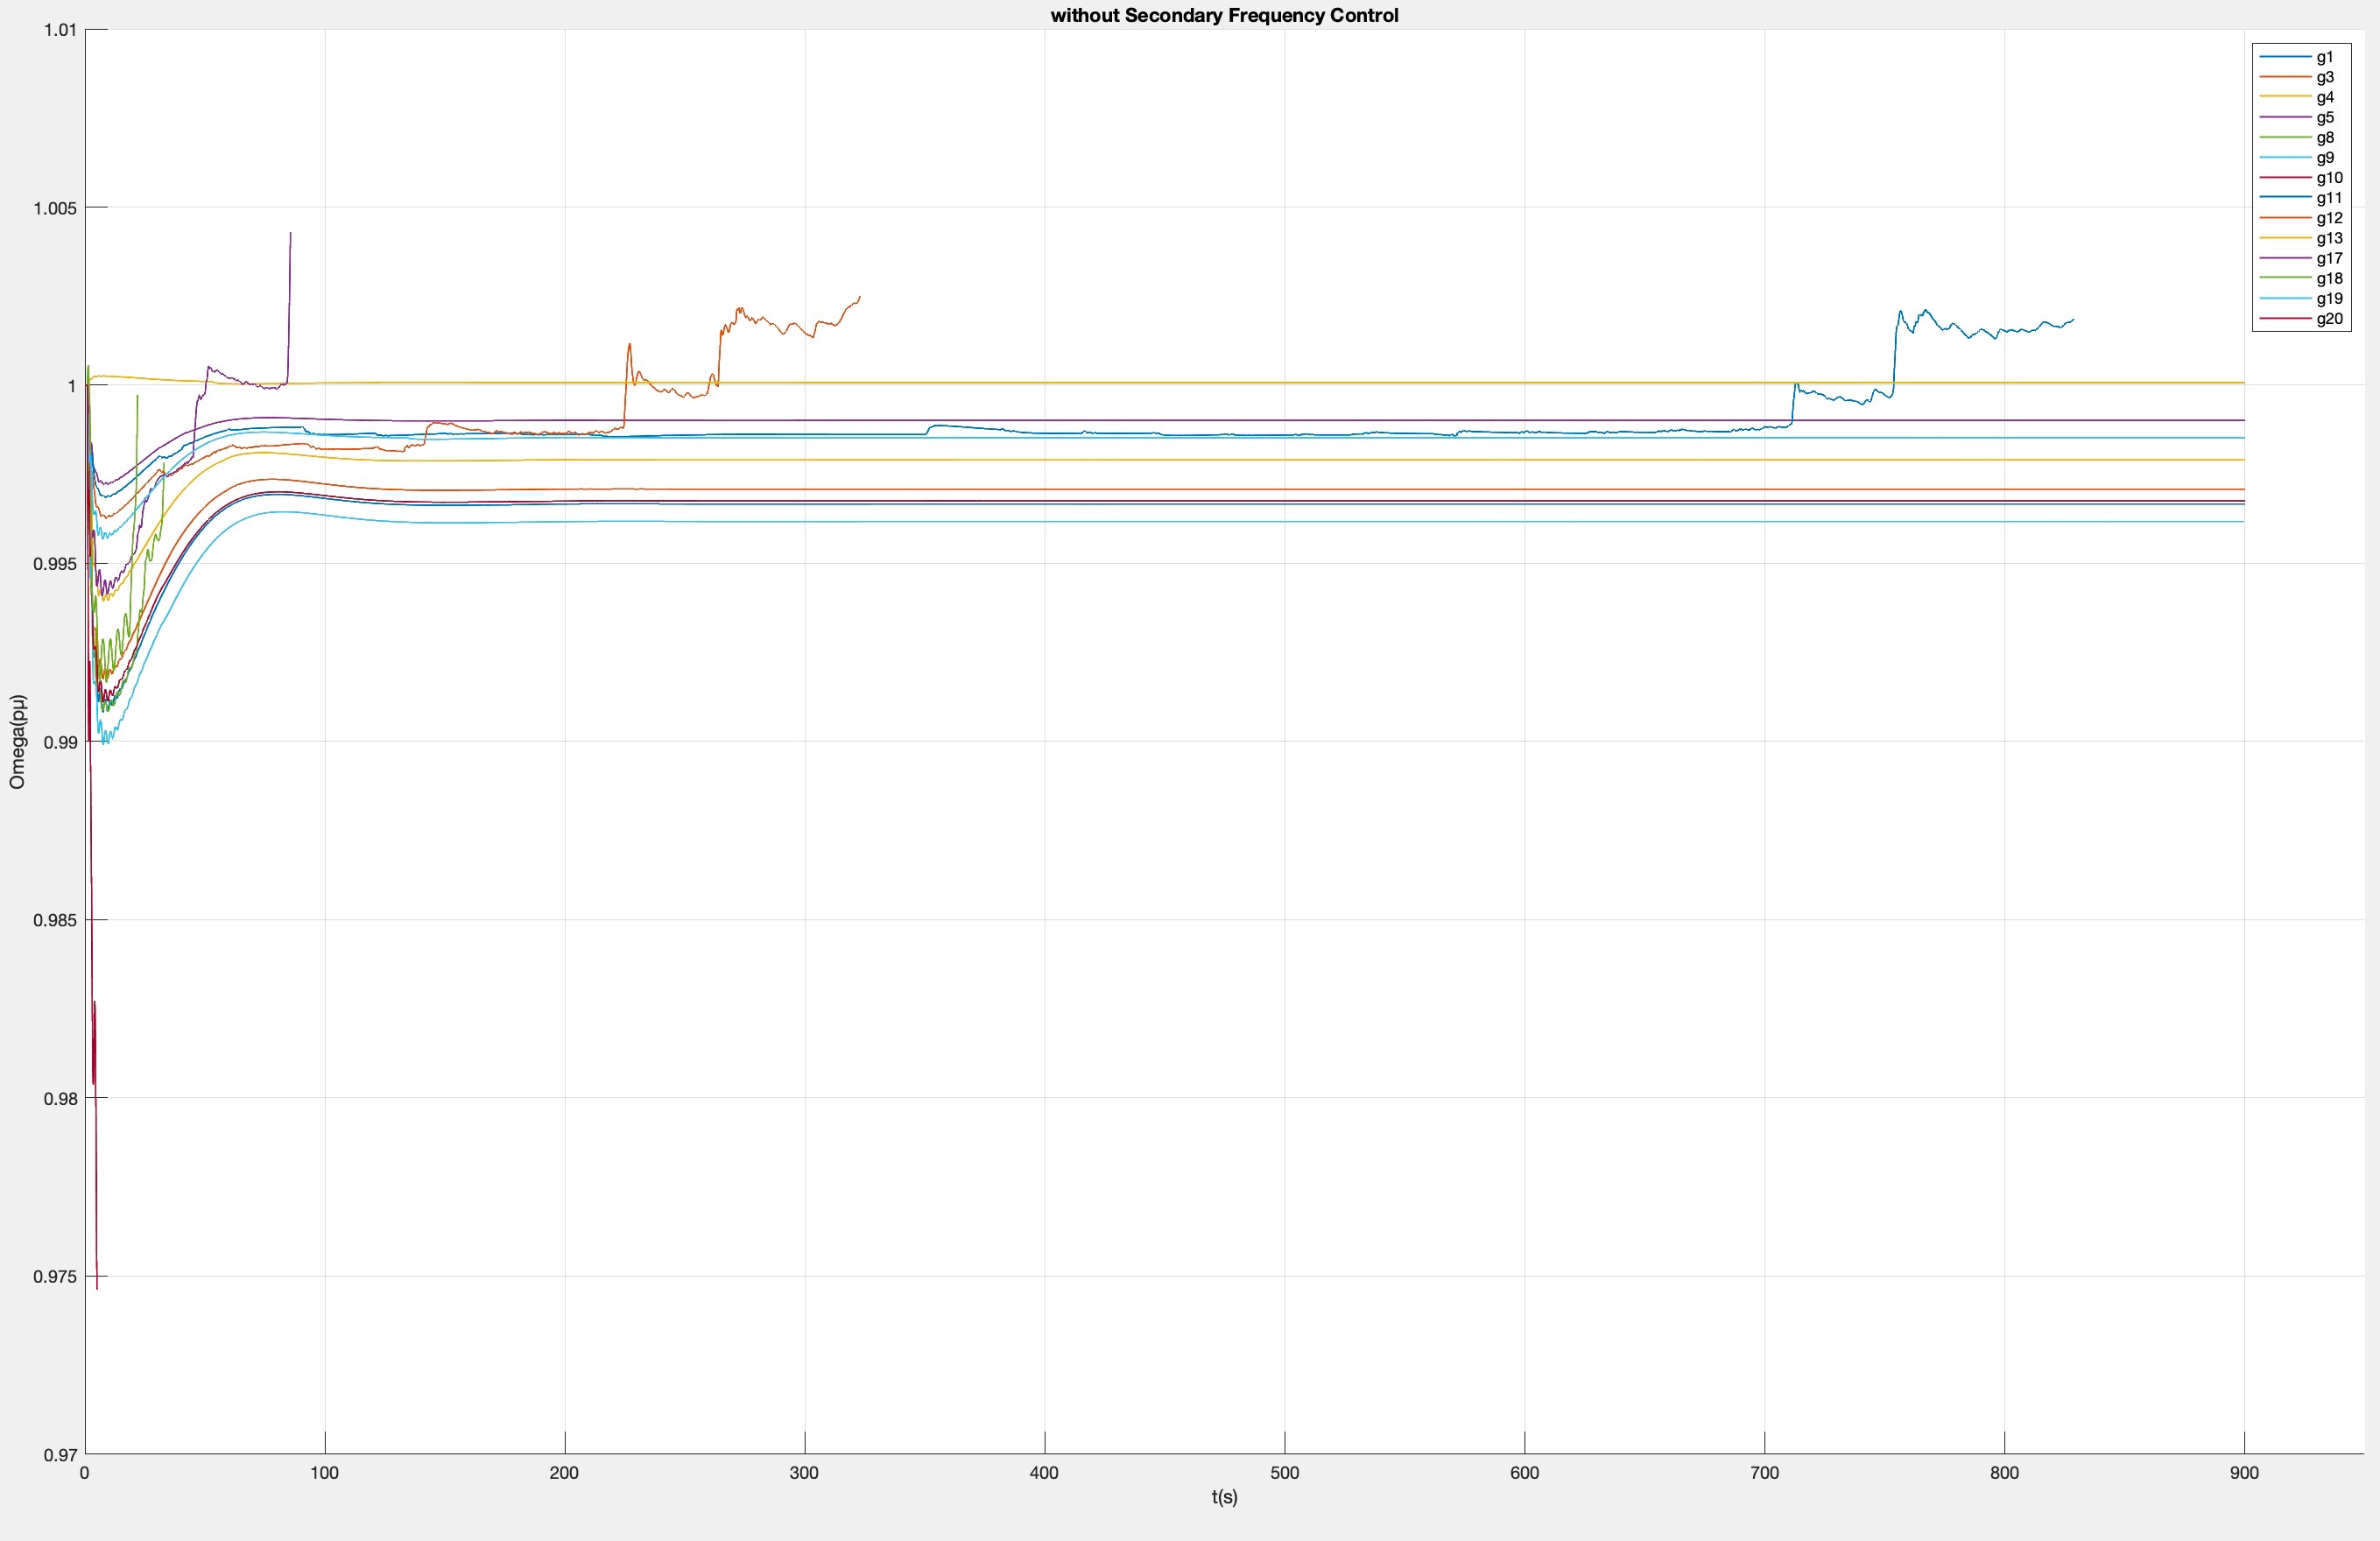
\includegraphics[width = .891\textwidth]{figure/4_1_1_without1.jpeg}
\caption{MATLAB figure: simulation results with different breakers, without SFC.}
\label{4_1_1_without1}
\end{figure}

As we can see from Figure~\ref{4_1_1_without1}, g8, g17, g18 and g20 are extremely unstable before 100 seconds and g13 have zero nominal power (because it has zero nominal power, from Table~\ref{nominalPower}). Thus, we choose a breaker out of them to make sure we have a smooth testing environment. 


\begin{figure}[htbp]
\centering
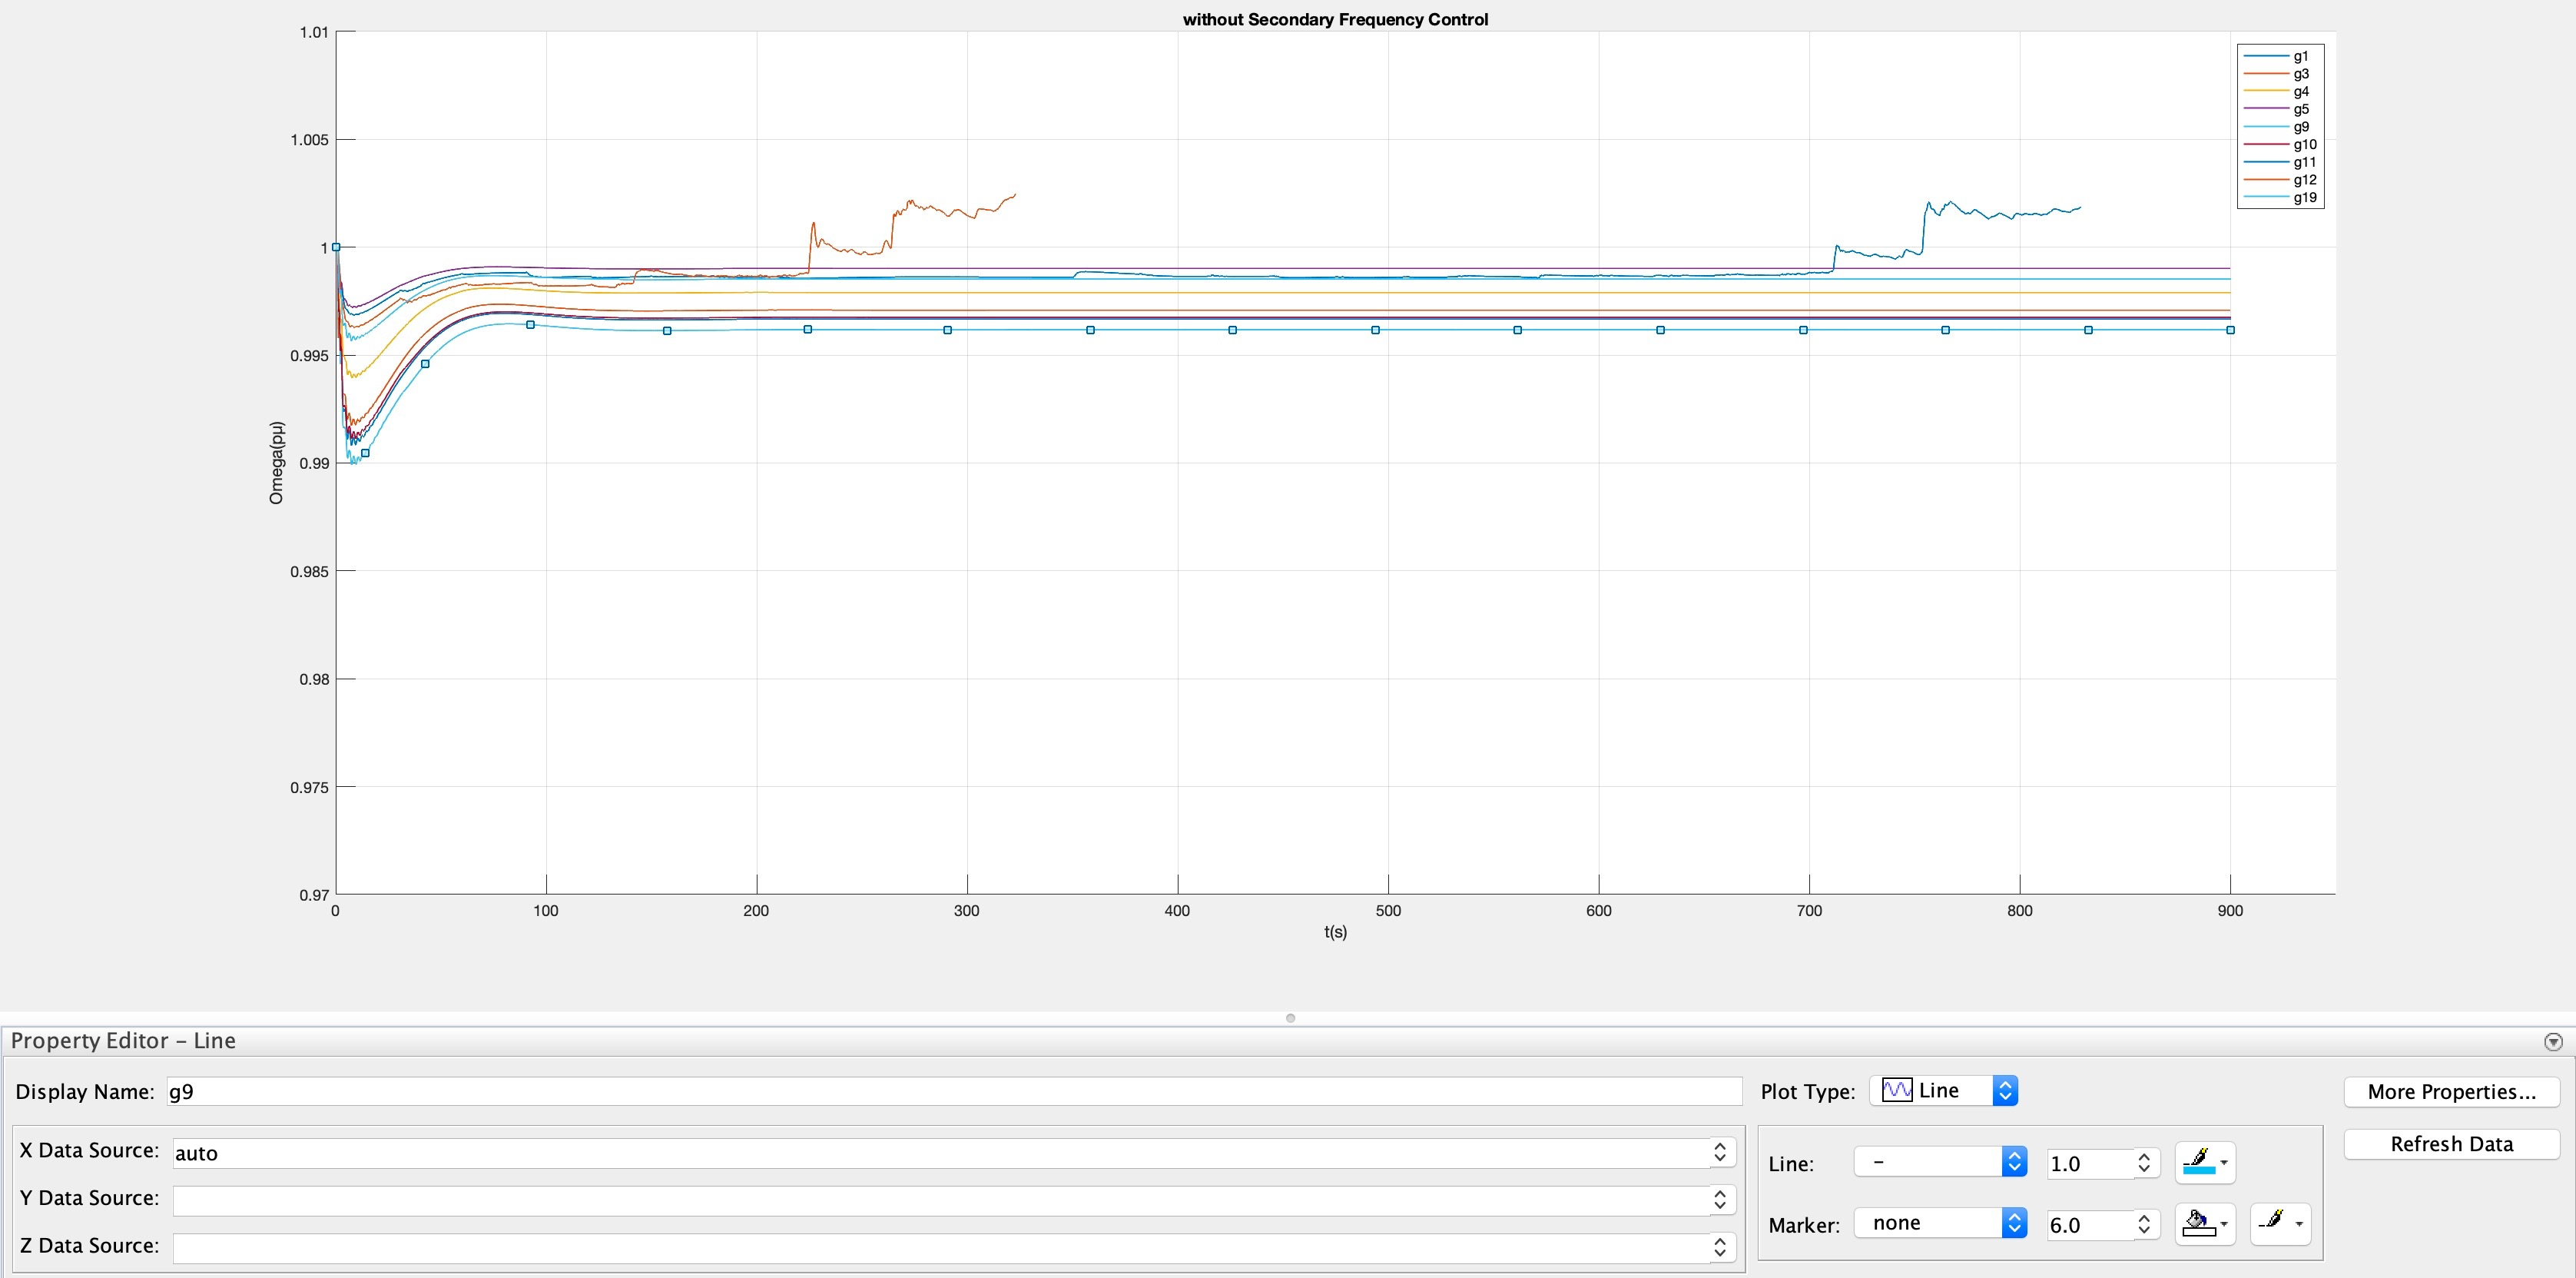
\includegraphics[width = .891\textwidth]{figure/4_1_1_without2.jpeg}
\caption{MATLAB figure: choose g9 as breaker.}
\label{4_1_1_without2}
\end{figure}

Finally, we choose g9, as shown in Figure~\ref{4_1_1_without2}, because it has a large steady-state error. Thus, the turbines will send more power to the system. It is easier to see the changes of kp and ki. 

\subsection{Software Hypothesis} %4.1.2

\begin{figure}[htbp]
\centering
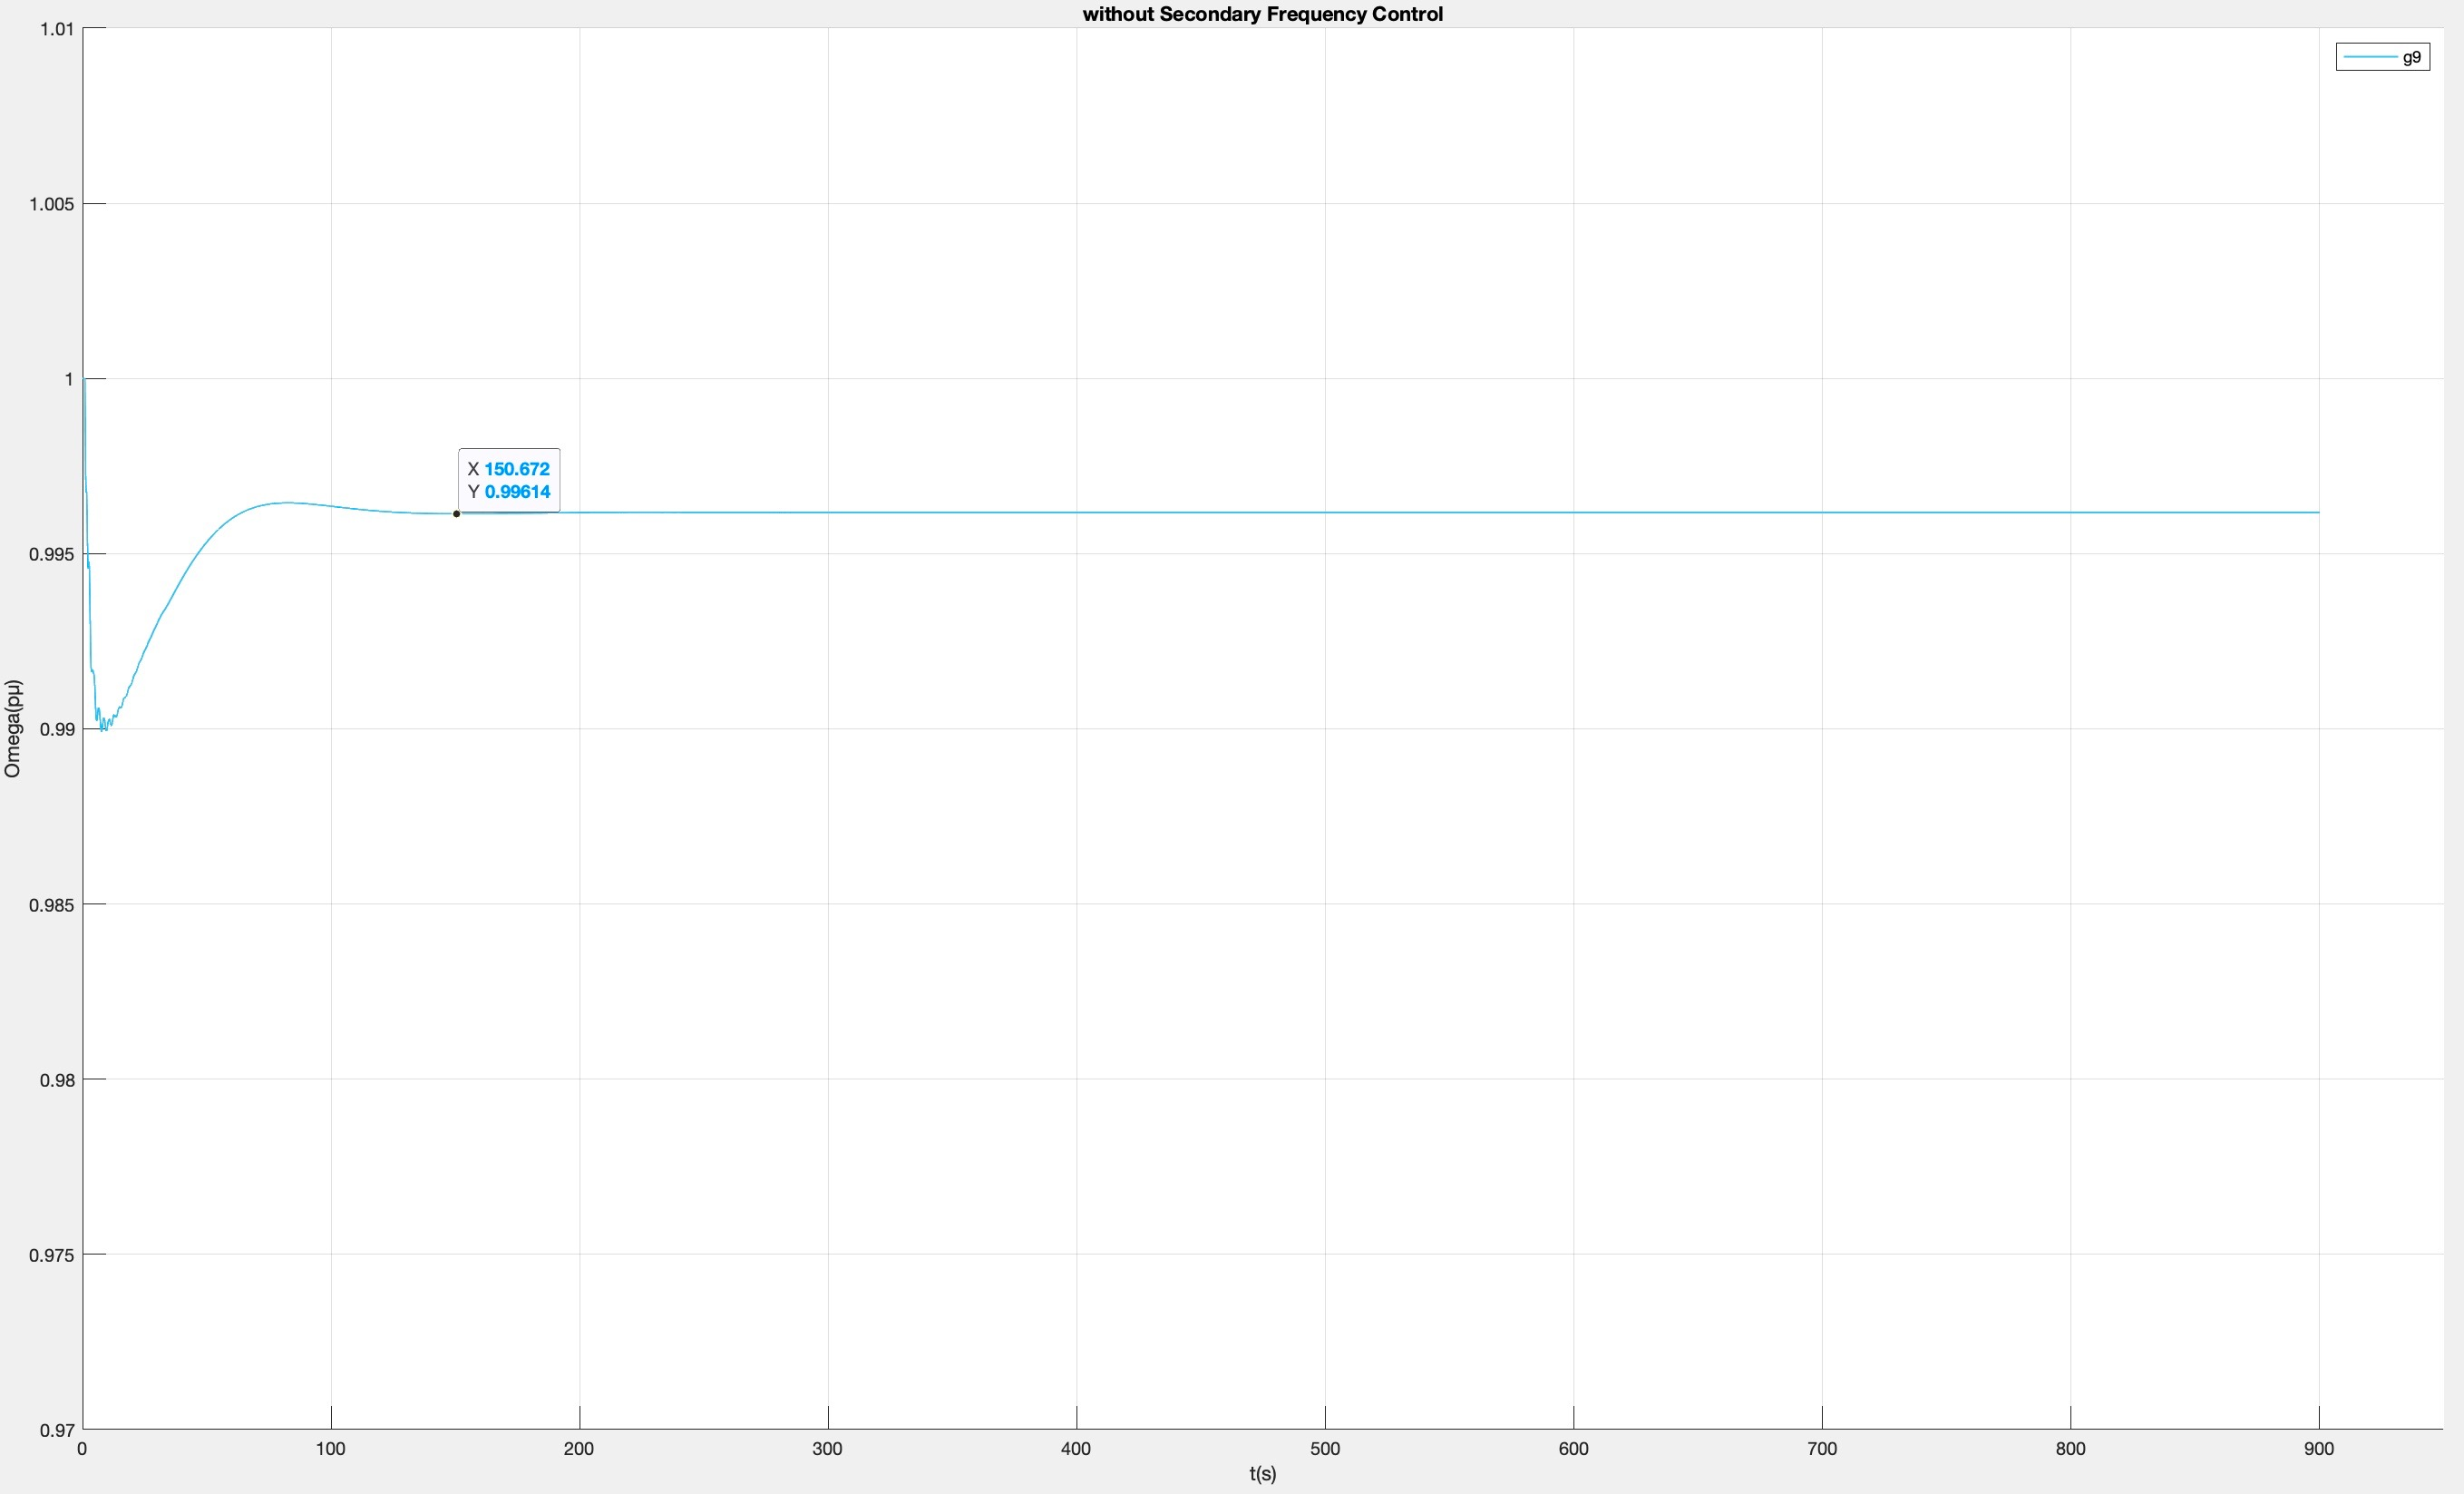
\includegraphics[width = .891\textwidth]{figure/4_1_1_without3.jpeg}
\caption{MATLAB figure: choose start time for SFC.}
\label{4_1_1_without3}
\end{figure}
Next hypothesis is about start time and end time. In the definition of Primary Frequency Control, its power balance will be restored at a lower or higher frequency, thus, from the Figure~\ref{4_1_1_without3}, we can observe that, at the 150th seconds, the frequency is stable. Thus, I choose the 150th second at the beginning of Secondary Frequency Control. In the definition of Secondary Frequency Control, the response time will take up to 15 minutes, thus, I choose the 900th second as my temporary end time. 

Since it is a low time delay testing, we can assume that delay is 0.01 seconds. The reason for not choosing idea situation (i.e. delay = 0 sec) is that, in reality, there be no such a zero delay scenario. 

Next step, we need to start tuning kp and ki. Following the idea of section~\ref{section3.4}, firstly, we assume a large value as a limit value of kp. Detailedly, we assume the range of kp and ki are both from 0.1 to 300.1 and their steps are both 50.  

Then, we use the designed MATLAB program to check whether the simulation results are acceptable. Detailedly, we set overshoot is smaller than 0.2 percent because it is required that the frequency error should be in range of ±0.1 Hz from Section~\ref{subsection4.1.1} in the Nordic official document. 

We also need to make sure the signal is really settled from 0.9998 to 1.0002 before the end time (i.e. the 900th second), thus, it is necessary to extend the simulation time and give the program more data to check whether it's settled before 15 minutes. Thus, we set 1000 sec as our end time.

Finally, the program sketches the plots of all the acceptable results and gives related information in the legend bar.\\

\begin{figure}[htbp]
\centering
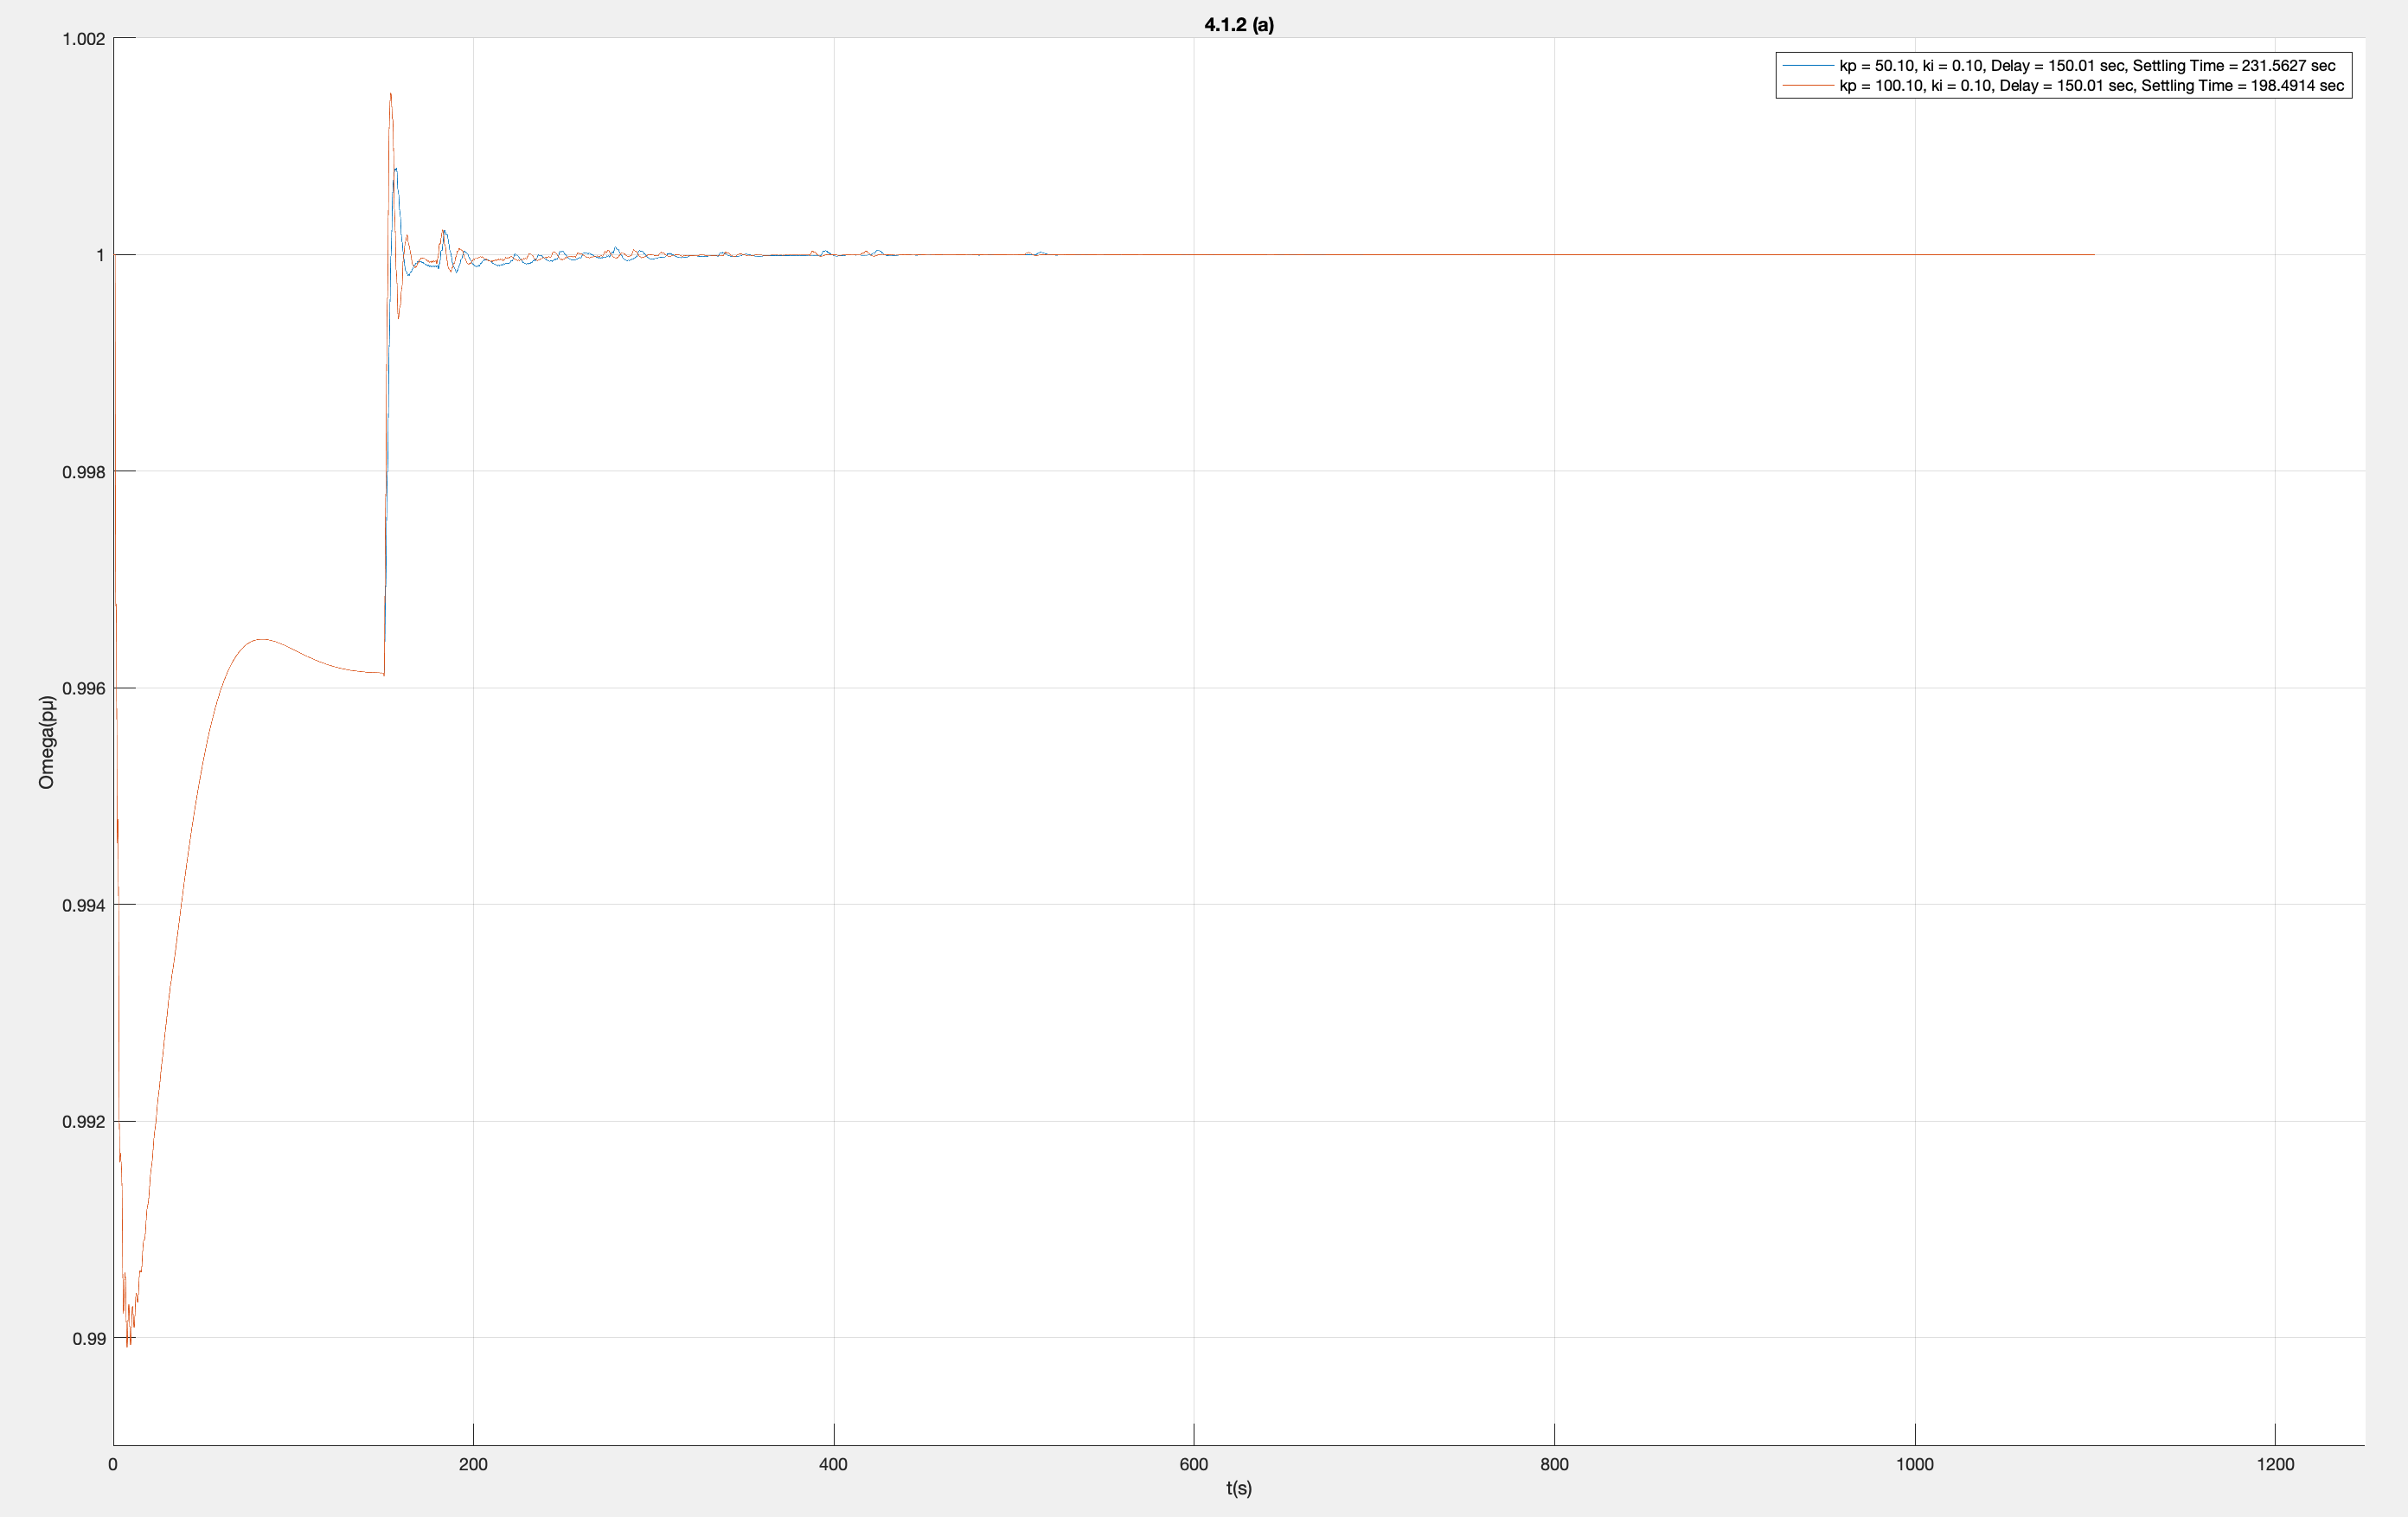
\includegraphics[width = .819\textwidth]{figure/4_1_2_a.png}
\caption{Disconnect generator g9: delay = 0.01 sec; kp: from 0.1 to 300.1 (step: 50); ki: from 0.1 to 300.1 (step: 50); start time=150s, end Time=1000s, required settling time=900s.}
\label{4_1_2_a}
\end{figure}

However, as you can see from Figure~\ref{4_1_2_a}, only two of all the simulations are acceptable. The maximum value of kp is 100.1 and the maximum value of ki is 0.1.  

According to the regulations from the last chapter, we need to increase the maximum amplifier factor by the step value.  

For instance, the new range of kp is between 0.1 and 150.1 and the new range of ki is between 0.1 and 50.1. To make more accurate results, we need to decrease the step at the same time. We set step be 10.0.  

Finally, we have another plot as shown in Figure~\ref{4_1_2_b}.  

\begin{figure}[htbp]
\centering
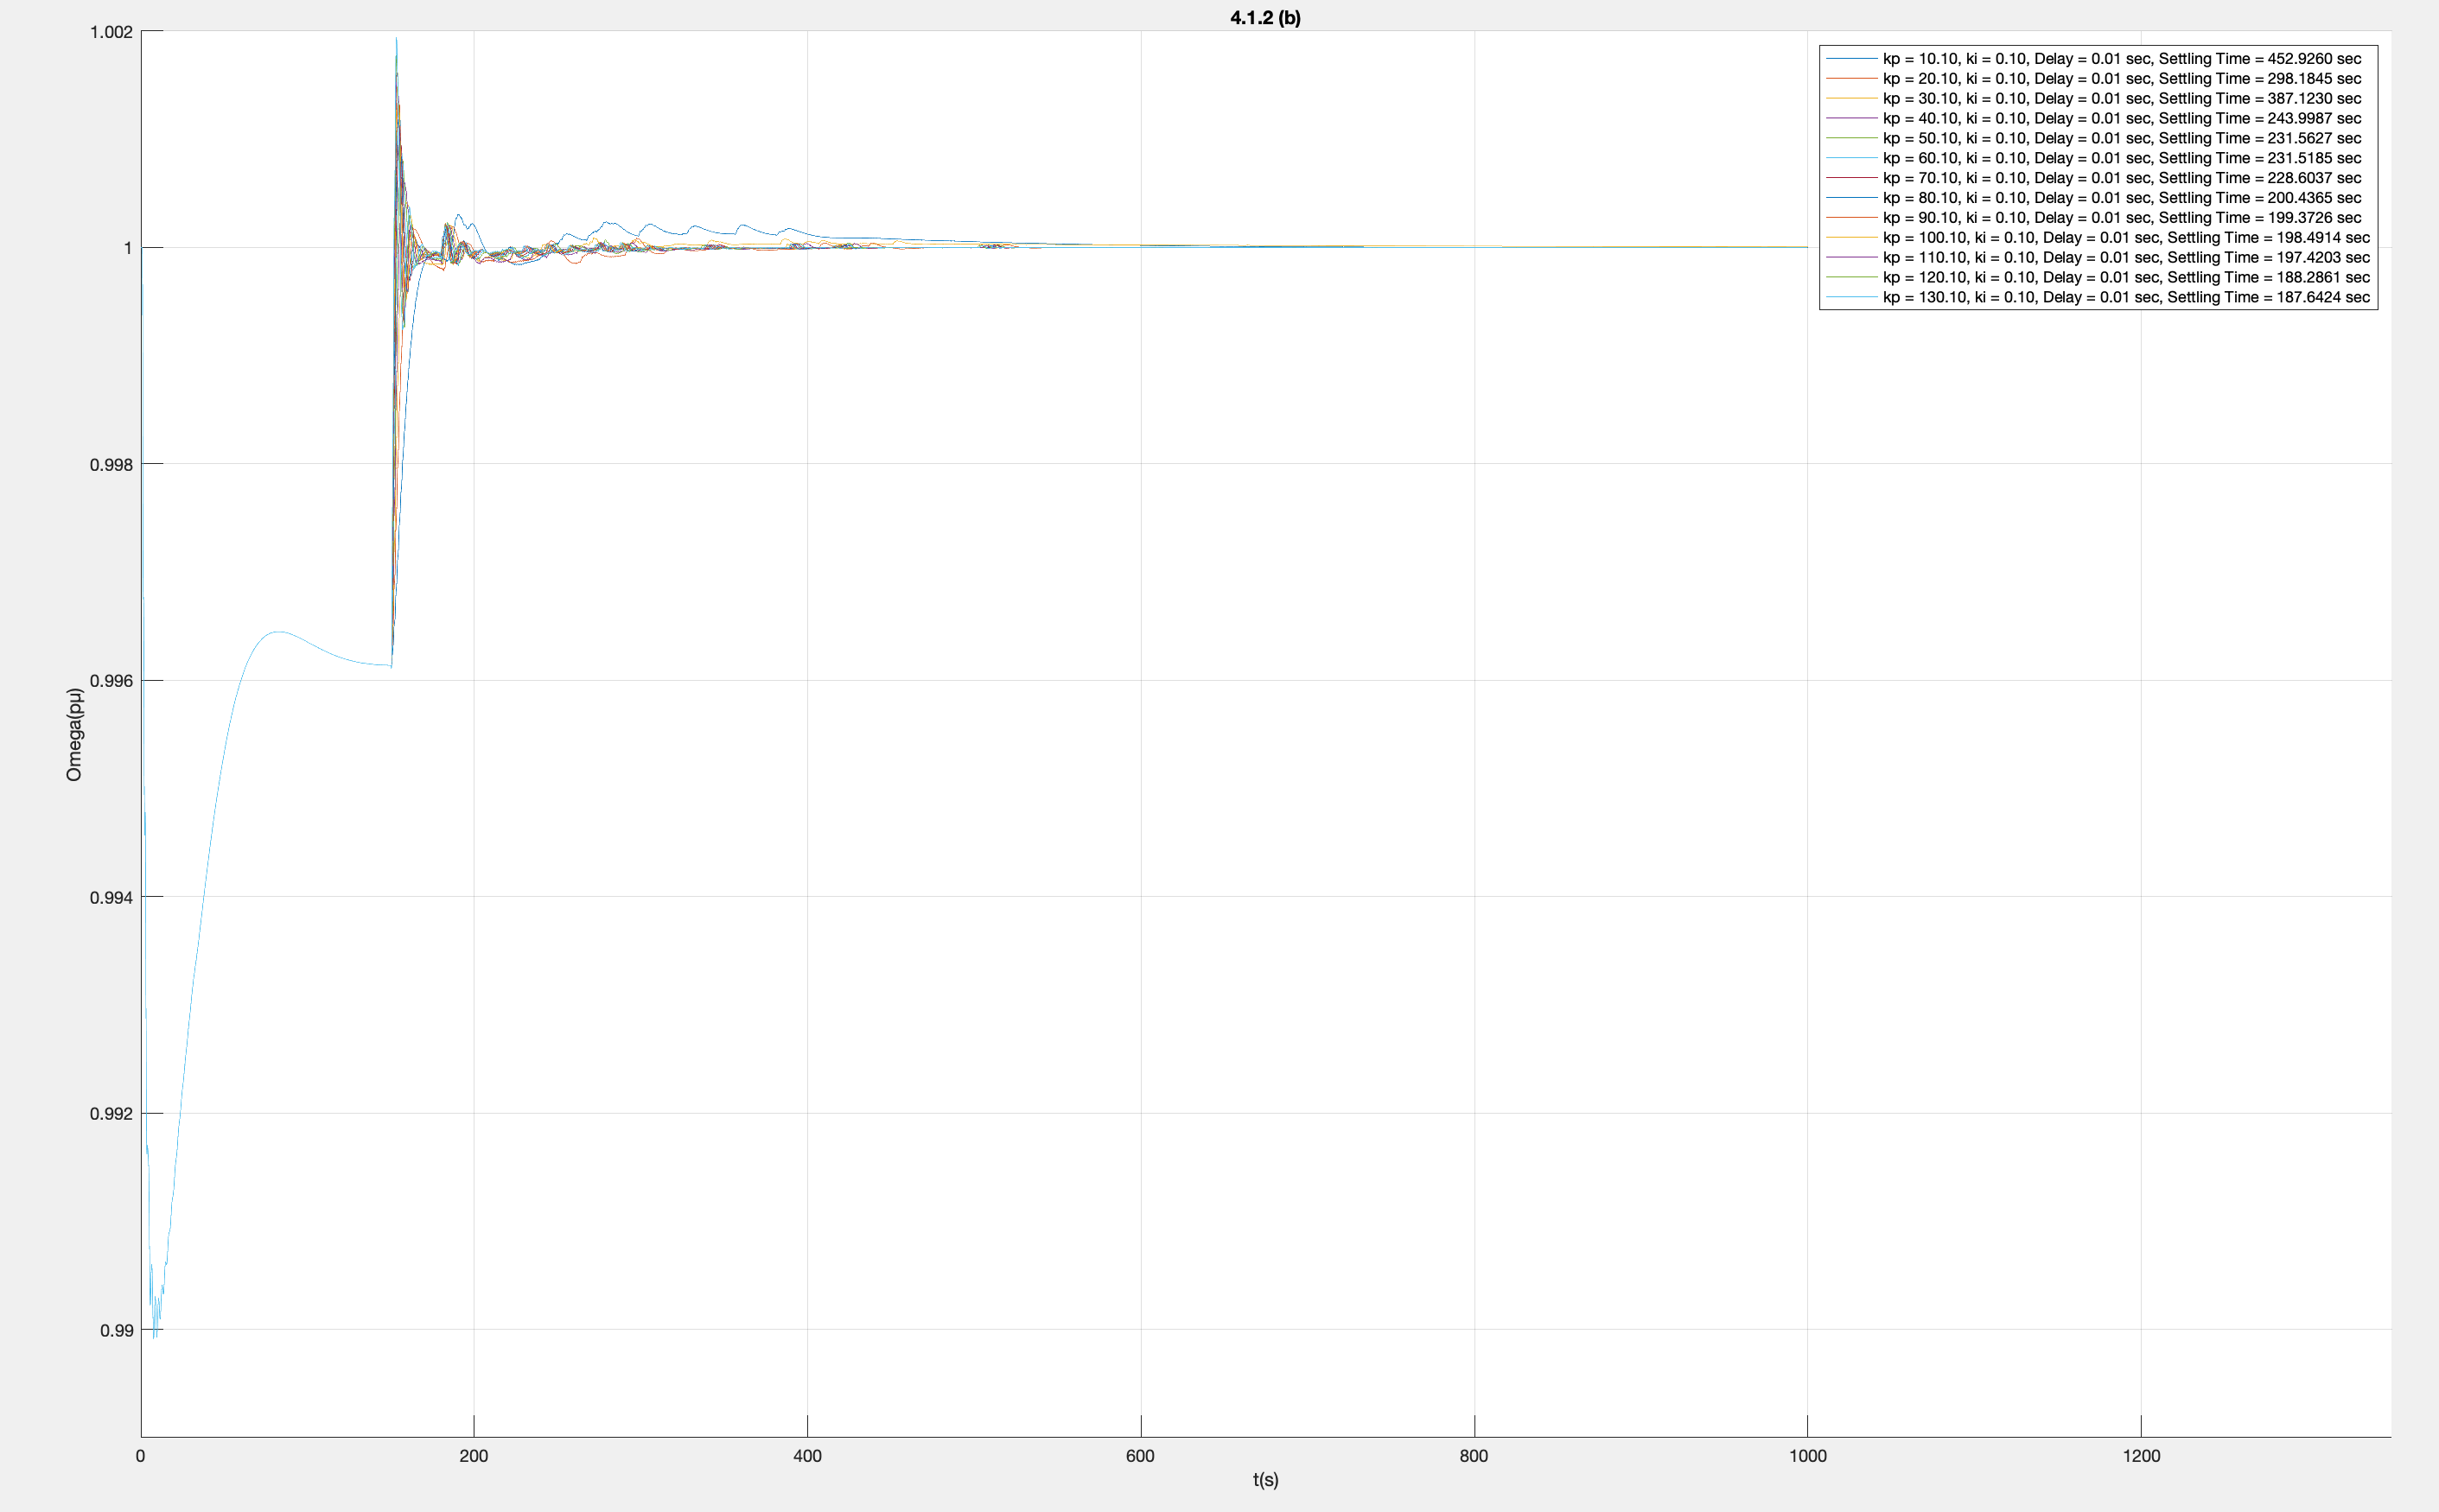
\includegraphics[width = .819\textwidth]{figure/4_1_2_b.png}
\caption{Disconnect generator g9: delay = 0.01 sec; kp: from 0.1 to 150.1 (step: 10); ki: from 0.1 to 50.1 (step: 10); start time=150s, end Time=1000s, required settling time=900s.}
\label{4_1_2_b}
\end{figure}


Apparently, we have more acceptable results than last simulation because of shrinking the step of kp. We find that the simulations are unacceptable if kp equals to 140.1 or 150.1. Thus, we can finally fix the range of kp between 0.1 and 140.1 and keep the step of kp to 10. We can set ki in a range of 0.1 and 10.1 with the reason above. However, it is possible that the maximum value of ki is still 0.1 if we set the range of ki be from 0.1 and 10.1. If so, then the simulations are meaningless.  

Thus, we need to apply bisection method on the range of ki and find the meaningful maximum ki. Detailedly, we range kp from 0.1 to 140.1 and set ki equals to 5.1. The purpose of doing this is to find whether there are acceptable results if ki is in the middle of 0.1 and 10.1.

The filtered results are as Figure~\ref{4_1_2_c}.  

\begin{figure}[htbp]
\centering
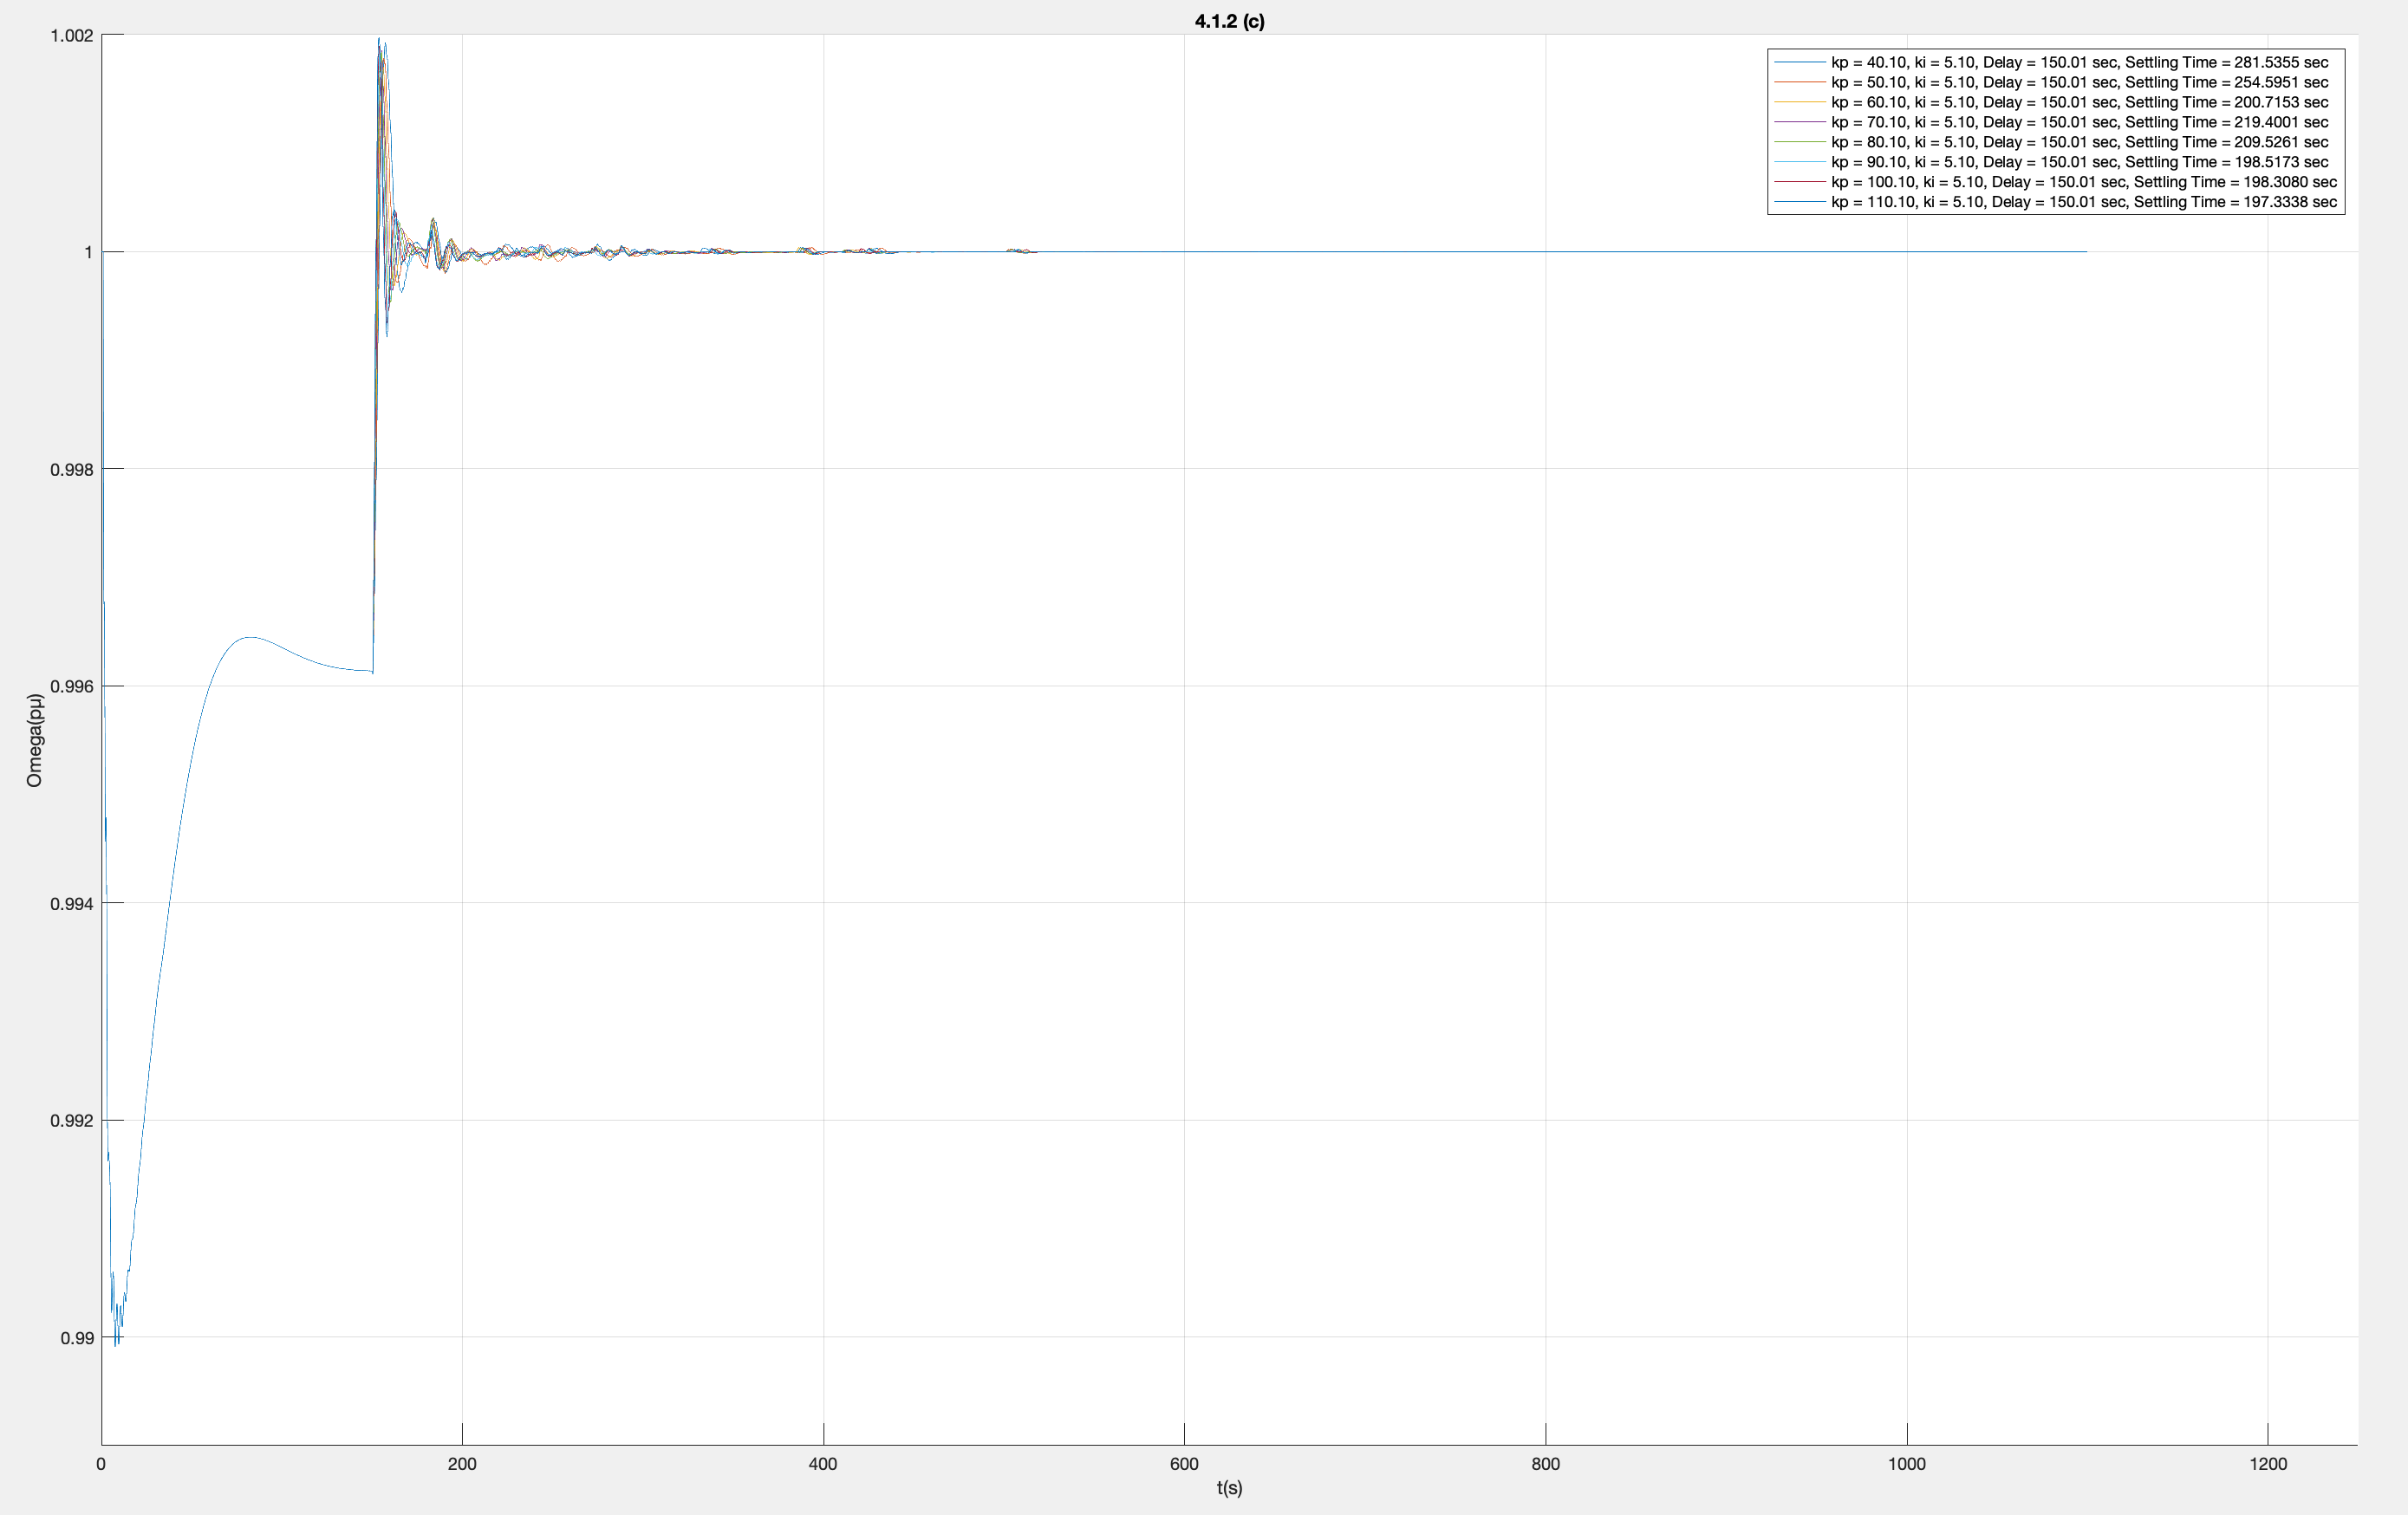
\includegraphics[width = .819\textwidth]{figure/4_1_2_c.png}
\caption{Disconnect generator g9: delay = 0.01 sec; kp: from 0.1 to 140.1 (step: 10); ki = 5.1; start time=150s, end Time=1000s, required settling time=900s.}
\label{4_1_2_c}
\end{figure}

The results shows there are acceptable simulations if ki equals to 5.1. \\

Thus, we can set the range of kp between 0.1 to 140.1 (step: 10.0), the range of ki between 0.1 and 10.1 (step: 1.0). The controller will start from 150 seconds and will end at 1000 seconds. We hope the signal can be settled before 900 seconds.